\section{Introduction}\label{sec:introduction}

As 6G networks process toward edge deployment, huge machine type communication, and network
slicing, the web attacks surface for web-oriented threats increases rapidly. Edge nodes process
latency with limited security instrumentation where data are increasingly served at the network
edge rather than centralized data centers. Safeguarding from web-based attacks such as brute force,
SQL injection and shell script exploitation with this setting requires a good architecture that is
accurate, lightweight enough for edge hardware and validate the ability to generalize across
traffic domains.

The increase in use of mobile devices have led to the rise of dependency on mobile networks and in
as a result escalated web-based attack. With the emergence of next generation 6G networks and the
growth of edge-based content sharing, security challenges are amplified. According to the report
of Edge-scan, mobile network-based vulnerabilities and web attacks have surged drastically since
the year 2023. Among the most well-known web attacks are brute force, shell script, and SQL
injection. As mobile traffic continues to dominate the internet usage globally [1], protecting
these networks, especially in the context of 6G edge deployments, has become very important. The
mobile environment not only have increased the attack surface in traditional web attacks [2] but
also have opened new security challenges related to distributed edge computing [3]. Deep learning
(DL) techniques are being applied across various cybersecurity areas like infrastructure threats
and attacks, software attacks, and privacy preservation [4].

\subsection{Main contribution of the research}\label{sec:contribution}

The goal of this research work is:

\begin{itemize}
  \item This research introduces a novel intellectual security architecture (ISA) that combines a
        lightweight Bi-LSTM temporal encoder with a transformer-based MHA model, specifically
        designed for detecting web attacks.
  \item To conduct a controlled ablation study separating the accuracy contribution of each
        component like Bi-LSTM only, MHA only, and hybrid model quantifying the benefit of
        combining them in attack detection.
  \item To provide a system level characterization such as parameter count, disk footprint,
        inference latency, and throughput for edge deployment feasibility;
  \item To perform exhaustive evaluation using a diverse dataset on trained model zero shot on an
        independent edge IIoT dataset reporting its strength as preserved AUC and limitation
        reduced accuracy on domain shift.
\end{itemize}

\subsection{Literature review}\label{sec:literature}

In recent years, the detection of web attacks in mobile networks is attracting the attention of
the researchers. To enhance security in mobile networks, and specifically in the context of
edge-based content sharing in next generation 6G networks, numerous ML and DL approaches have been
proposed in the literature.

Tian et al. [9] proposed a hybrid model which combines long short-term memory (LSTM) and
convolutional neural networks (CNNs) for web attack detection. To identify the malicious patterns,
they processed HTTP request as character sequences and then extracted both the temporal and spatial
features. Their approach demonstrated 98.2\% accuracy with a false positive rate of 0.76\% that was
tested against five types of web attacks. Although while dealing with unknown attack types like
zero-day attack, their accuracy reduced to 12\% which shows the limitation of the model while
dealing with the dynamic mobile environment.

Zhang et al. [10] introduced a network intrusion detection system (NIDS) combining Bi-LSTM and
multihead attention mechanism. An embedding layer was used to convert input features into dense
vector and then the multi-head attention assigned different weights to various parts of the input
sequence in a way enhancing the focus of the model on critical features. They evaluated their model
on datasets namely KDDCUP99, NSLKDD, and CICIDS2017 that recorded accuracies of 98.29\%, 95.19\%,
and 99.08\%, respectively. Due to the inherent properties of mobile environments, particularly
resource constraint and real-time processing capabilities (critical in edge deployments), the
proposed model's applicability to mobile networks remains unexplored.

\subsection{Research gap}\label{sec:gap}

The above-mentioned literature classifies the following methodological gaps, which are
particularly pronounced in next generation 6G and edge-based content sharing environments:

\begin{enumerate}
  \item Many traditional models of web attack detection are based on heavy and deeper architecture
        models, which are not suitable for edge devices and resource-constrained computing
        environments.
  \item Current deep learning models are slow in detecting real-time web attacks and provide
        overfitting results with high classification accuracy on imbalanced multiclass attack
        datasets, making them unsuitable for the high-speed, dynamic nature of 6G traffic.
  \item Most models are black boxes that do not consider important data such as HTTP requests and
        URL mapping. This results in poor interpretability of the predicted outcomes, which is
        vital for forensic analysis within an Intellectual Security Architecture (ISA).
\end{enumerate}

\subsection{Methods and experiments}\label{sec:methods}

The proposed research is to predict the different types of web attacks in next generation 6G
mobile communication networks, which may stall the efficiency of mobile networks with coverage
issues and low bandwidth in metropolitan areas, especially affecting edge-based content sharing.

\subsubsection{Material}\label{sec:material}

The dataset parameters used in the experiments are summarized in
Table~\ref{tab:dataset}.

\begin{table}[htbp]
  \centering
  \small
  \caption{Dataset parameters}
  \label{tab:dataset}
  \begin{tabularx}{\linewidth}{@{}lX@{}}
    \toprule
    Features & Testing data \\
    \midrule
    Traffic data & Source and destination IP \\
    Headers & HTTP, URL \\
    Payload & Content, query, token \\
    Network info & Port, packet size, duration \\
    Training and validation set & 70:30 \\
    Label & Bots, DDoS, DOS, Port scanning, Web attacks -- Brute force, SQL injection \\
    \bottomrule
  \end{tabularx}
\end{table}

\subsubsection{Dot product attention}\label{sec:attention}

After using the attention function as the first step to change the dimensions of each head from the
initial layer to capture long-range dependencies, create a foundation for dot product attention,
shown in Eq.~\eqref{eq:attention}:

\begin{equation}
  \operatorname{Attention}(Q,K,V)
  = \operatorname{Softmax}\left(\frac{QK^{\top}}{\sqrt{d_k}}\right)V,
  \label{eq:attention}
\end{equation}

where \(d_k\) are the dimensions of key vectors inside the attention layer with activation
function.

\subsubsection{System model}\label{sec:system}

The next process after normalization is the pooling function, which reduces the length of each
sequence, like link address, HTTP request, and duration, to a fixed length. This is important for
creating compact feature vectors for the final classification layer within the intellectual
security architecture (ISA) [44]. The average pooling function removes the dimension of time to
make each sequence feature to enter the next dense layer as a fixed-size feature vector. The
equation of average pooling is expressed in Eq.~\eqref{eq:pooling}:

\begin{equation}
  \mathrm{RC}_1
  = \operatorname{ReLU}\left(W_1 \mathrm{RC}_{\mathrm{avg}} + b_1\right).
  \label{eq:pooling}
\end{equation}

\subsubsection{Query key value}\label{sec:query-key}

Finally, binary cross-entropy loss is used to train the model in an effective way to handle model
loss and prevent overfitting. The main advantage of this loss function is its ability to minimize
classification errors related to web attacks or normal operations within the mobile communication
network, which is essential for the reliability of the intellectual security architecture (ISA) in
6G edge nodes [46]. The final layer applies a SoftMax activation over seven output classes such as
normal traffic, bots, brute force, DDoS, DoS, Port scanning, and web attacks process a variable
distribution over attack types expressed in Eq.~\eqref{eq:softmax}:

\begin{equation}
  y = \operatorname{Softmax}\left(W_2 \mathrm{RC}_{\mathrm{avg}} + b_2\right).
  \label{eq:softmax}
\end{equation}

Given the severe class imbalance across the seven categories, the model is trained with class
weighted sparse categorical cross-entropy expressed in Eq.~\eqref{eq:loss}:

\begin{equation}
  \mathrm{Loss}
  = -\sum_{c=1}^{7} w_c y_c \log\left(\hat{y}_c\right),
  \label{eq:loss}
\end{equation}

where \(w_c\) is the weight applied to class \(c\).

\subsubsection{Architecture and algorithm}\label{sec:architecture}

Fig.~\ref{fig:architecture} defines the conceptual model of the proposed intellectual security
architecture (ISA) model.

\begin{figure*}
  \centering
  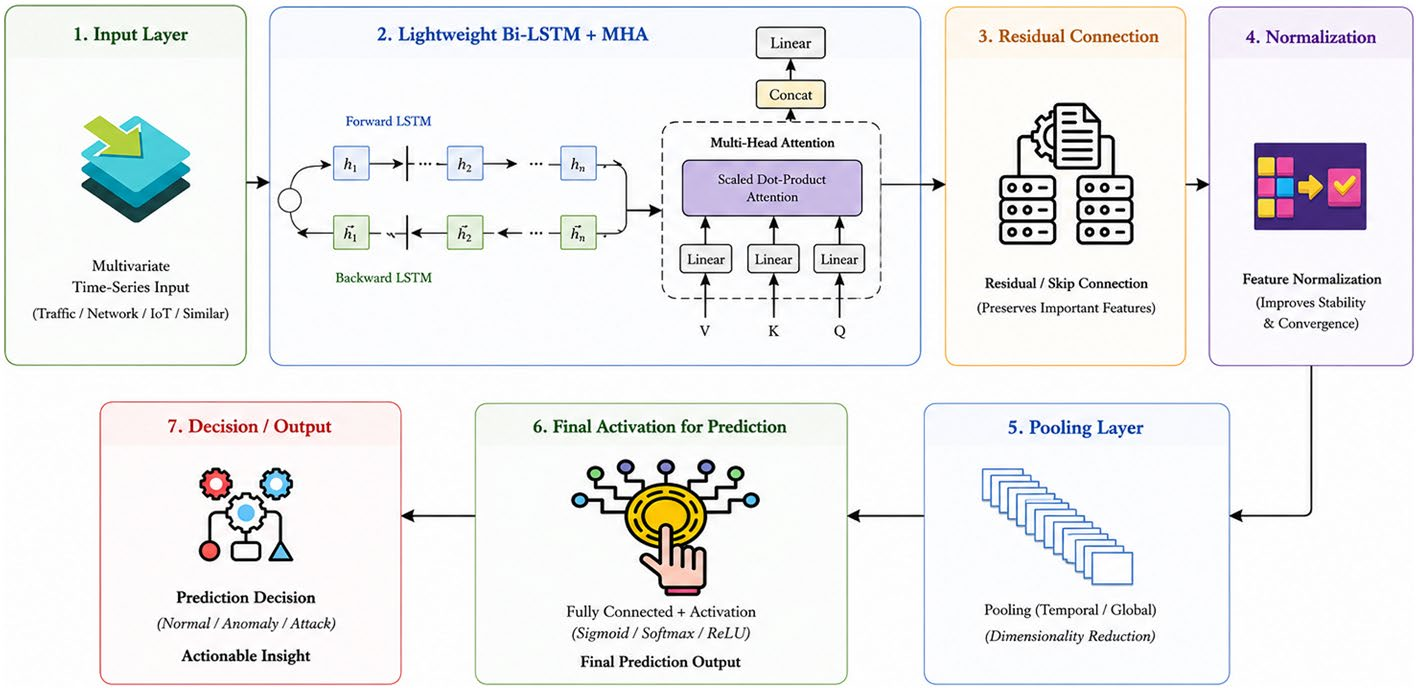
\includegraphics[width=\linewidth]{figure1}
  \caption{Conceptual visualization of the proposed intelligent attack detection framework.}
  \label{fig:architecture}
\end{figure*}

The process is to separate the class of each attack that is performed inside the mobile
communication network and this is most useful in imbalanced dataset.
Fig.~\ref{fig:roc} displays the AUC curve of the proposed work.

\begin{figure}
  \centering
  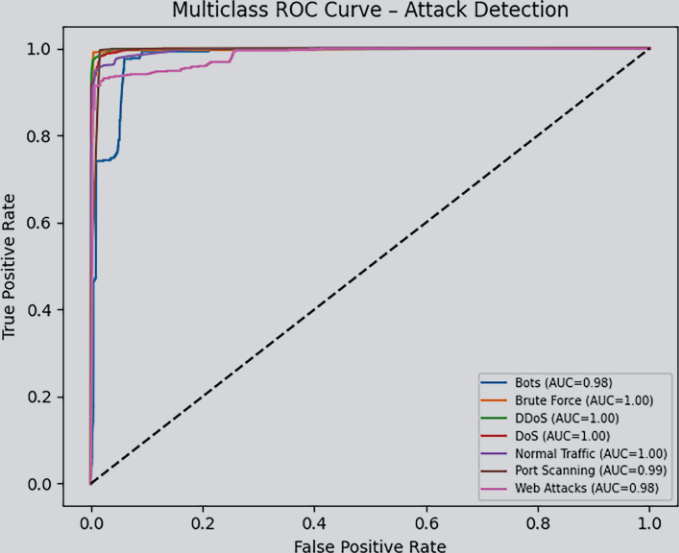
\includegraphics[width=0.9\linewidth]{figure2}
  \caption{Receiver operating characteristic (ROC) and area under curve (AUC) analysis for
           multiclass attack detection.}
  \label{fig:roc}
\end{figure}
